\documentclass[12pt]{report}

\usepackage{url}
%\usepackage[dvips]{graphicx}
\usepackage{graphicx}
\usepackage{amsmath}
\usepackage{longtable}
\usepackage{amssymb}
\usepackage[round]{natbib}
\bibpunct{(}{)}{;}{a}{,}{,}
\usepackage{cite}
\usepackage{longtable}
\usepackage{dcolumn}
\usepackage{siunitx}
\usepackage{lscape}

% If there are any other \usepackage commands, put them here.

\usepackage{guthesis} % Must be the last package

\newtheorem{theorem}{Theorem}[section]
\newenvironment{proof}[0]{\textit{Proof.}}{}
\newcommand{\qed}{\hfill $\Box$}

% To comment out multiple lines of text.
\long\def\comment#1{}

\title{The Effect of Electronic Health Records Adoption
on Patient-specific Health Education Prescription, Time Utilization, and Returned Appointments: A Propensity Score Weighted Analysis}

\author{Huade Huo}

\previousdegree{B.Mg.}

\thisdegree{Master of Public Policy}  % or Doctor of Philosophy, etc.

\thisdiscipline{Public Policy}

\thesistype{Thesis}     % or Dissertation

% defense or approval date, not today's date...
\thesisday{10}
\thesismonth{April}
\thesisyear{2015}

\professor{Yuriy Pylypchuk}
%\secondprofessor{Alonzo Church}   % Only if you have 2 major professors!

\fulltitle{The Effect of Electronic Health Records Adoption
on Patient-specific Health Education Prescription, Time Utilization, and Returned Appointments: A Propensity Score Weighted Analysis}

\indexwords{Electronic~Health~Records, Patient-specific Health Education, Time Utilization,
            Returned Appointments, Propensity Score Weighting, Theses~(academic)}

\begin{document}

\pagenumbering{roman}

\maketitle    % Creates title page, copyright page if any, and approval page.

\begin{abstract}
In this analysis, we use National Ambulatory Medical Care Survey data to investigate whether the adoption of the ambulatory electronic health records (EHR) system is associated with changes in patient-specific health education prescription rates, patient-physician interaction time, and returned appointment rates. We estimate the treatment effect of EHR adoption with multinomial propensity score weighting adjusted regressions. We find evidence to suggest that full EHR adoption positively affects patient-specific health education prescription rates. We find no robust evidence to show a significant effect of the EHR system on time utilization or returned appointment rates. We discuss possible reasons for our findings. We recommend linking patient education with quality improvement efforts and improving the usability of EHR systems.
\end{abstract}



\pseudochapter{Acknowledgments}
First, I offer my sincerest gratitude to my thesis advisor, Dr. Yuriy Pylypchuk, who has supported me throughout my thesis, for his patience, optimism, enthusiasm, and immense knowledge. I thank him for his systematic guidance, critical comments, and great effort in training me in the health policy research field. Without his guidance, mentoring, and support, this study would not have been completed. One could not wish for a better or friendlier thesis advisor.

I am thankful to Dr. William Gormley, Dr. Deborah Phillips, Dr. Sara Anderson, and other outstanding colleagues at the Center for Research on Children in the United States (CROCUS). They have provided generous support on my thesis, with their expertise, flexibility, and encouragement. I also thank Dr. Elizabeth Stuart from Johns Hopkins University for her excellent workshop on propensity score techniques at the CROCUS. Her detail-oriented guidance on my thesis has made this a thoughtful and rewarding journey.

I thank Dr. Barbara Schone, Dr. Carolyn Hill, and Dr. Michael Bailey for their incredible lectures that introduced me to intermediate econometrics methodologies. They have supported me academically and emotionally through my journey at the McCourt School. I thank Dr. Ali Arab from the Department of Mathematics and Statistics for enrolling me in his mathematical statistics class with waived prerequisites and providing detailed advice on statistical methods. The completion of this thesis would not have been possible without them.

In my daily work, I have been blessed with friendly and cheerful McCourt faculty, staff, classmates, and alumni. Thank you for all that you have taught me. I thank my friends for continuing to give, even when I had nothing to give in return.

Last but not least, I would like to thank Huanjun Zhang. She was always there cheering me up and stood by me through the good times and bad. I would also like to thank my parents. They have always supported me and encouraged me with their best wishes. Without all their love, I would not be able to do anything.

Notwithstanding all of the above support for my thesis, any errors and/or omissions are solely my own.

\tableofcontents

\listoffigures  % Optional - Omit this line if you don't want a list of figures.
\listoftables   % Optional - Omit this line if you don't want a list of tables.

\newpage

\pagenumbering{arabic}  % Ordinary pages have Arabic numerals.
\chapter{Introduction}
The United States spent 17.9\% of GDP on health expenditure in 2012 \citep{wbgHealthGDP}, and the figure is continuing to grow. Some scholars propose that one way to improve health care efficiency and quality is to adopt the electronic health records (EHR) system. President Barack Obama’s administration has prioritized the improvement in quality and efficiency of the health care system with the EHR system and launched Medicare and Medicaid EHR incentives for the adoption and use of the EHR system. The adoption rate of the EHR system increased rapidly; in 2013, ``more than half of eligible providers -- doctors, dentists and other eligible providers -- have qualified for and received incentive payments for adoption of certified electronic health records.'' \citep{whitehouseblogintro}

However, the empirically measured effect of adopting the EHR on quality or efficiency improvement is still very limited. Limited research has evaluated the effect of EHR adoption on quality or efficiency improvement at the national level. Even less analysis has provided an investigation on the adoption of the EHR system on patient-specific health education prescription or returned appointments using national data. Given the increasing adoption of the EHR and the implementation of EHR incentive programs, the effect of the EHR on these health outcomes is of interest.

In this analysis, we use National Ambulatory Medical Care Survey (NAMCS) data to investigate the effect of EHR adoption on three outcomes: patient-specific health education prescription rates, patient-physician interaction time, and returned appointment rates. The NAMCS is a national survey with extensive information at visit-level or physician-level, including whether the physician practice has an EHR system, health education prescription status, the breakdown of patients by different payment types, time spent with a physician for each visit, whether the visit is a returned appointment, and so on.

We estimate the treatment effect of EHR adoption with multinomial propensity score weighting adjusted regressions. First, we estimate the multinomial propensity score using generalized boosted models (GBM)  developed by RAND \citep{mccaffrey2013tutorial}. Second, we examine whether the propensity score assumption is satisfied and assess the balance statistics before and after propensity score weighting. The propensity score overlap assumption meets and the balance statistics are (at least) acceptable. Third, we use the estimated multinomial propensity score as weighting in regression models. To achieve ``double robustness,'' the regression model includes covariates that exceed a threshold of the balance statistics. Finally, we test the sensitivity of our result with different model specifications.

We find evidence to suggest that full EHR adoption positively affects patient-specific health education prescription rates. Physicians are expected to increase patient-specific health education prescription rates by 3.4\% if they fully adopt the EHR system ($t=1.89$). We find no robust evidence to show a significant effect of the EHR system on time utilization or returned appointment rates.

In what follows, we discuss possible reasons for our findings. The ease of use of the EHR system, the requirement of the EHR incentive program, and other hypothetical reasons possibly contribute to these findings. However, our research design does not allow us to identify the casual mechanisms for these results. We recommend linking patient education with quality improvement efforts and improving the usability of EHR systems.

In this paper, Chapter \ref{chapter:lit} reviews the policy background and literature, Chapter \ref{chapter:analysisplan} details the analysis plan for this research, Chapter \ref{chapter: desc} provides descriptive statistics of NAMCS data used in this analysis, Chapter \ref{chapter:psb} assesses the propensity score balance and assumptions graphically and numerically, Chapter \ref{chapter: reg} provides regression results, Chapter \ref{chapter:discussion} discusses possible reasons for the pattern of findings, Chapter \ref{chapter:limitations} summarizes the limitations of this research, Chapter \ref{chapter:policyimplications} provides policy implications, and Chapter \ref{chapter:conclusion} concludes the paper.


\chapter{Literature review}
\label{chapter:lit}
\section{Background}

In 2009, the US Congress passed the American Recovery and Reinvestment Act (ARRA), which appropriates funds to promote the adoption and use of health information technology (HIT). To promote the adoption and meaningful use of electronic health records among health care providers, ARRA authorized that ``\$1,500,000,000 shall be available for grants for construction, renovation and equipment, and for the acquisition of health information technology systems'' \citep{AARALaw}. 

The Centers for Medicare \& Medicaid Services launched the Medicare and Medicaid EHR Incentive Programs after the passage of ARRA in 2009. These programs provide incentive payments to eligible professionals, eligible hospitals, and critical access hospitals (CAHs) as they adopt, implement, upgrade or demonstrate meaningful use of certified EHR technology. In order to receive the EHR stimulus money, the HITECH act (ARRA) requires eligible physicians to show ``meaningful use'' of an EHR system.

Take the Medicare EHR incentive program as an example. Eligible physicians must attest yearly that they demonstrate meaningful use to receive the EHR incentive and avoid a Medicare payment adjustment. In order to demonstrate meaningful use in 2014 Stage 1, eligible professionals must meet 13 required core objectives and 5 menu objectives from a list of 9. The core objectives includes recording selected patient demographics, maintaining active medication lists, protecting electronic health information, etc. The menu objectives include using certified EHR technology to identify patient-specific education resources, sending patient reminders, and implementing drug formulary checks, etc. \citep{stage1}.

\section{Effect of EHR on health expenditure}

Limited empirical studies have estimated the potential net benefits that could arise from adopting health information technologies (HITs), especially at the national level. The RAND Corporation estimated that annual net savings to the health care sector from efficiencies alone could be \$77 billion or more based on surveys, publications, interviews, and an expert panel review \citep{Rand2005}. Hillestad et al. claimed that effective EHR implementation and networking could eventually save more than \$81 billion annually by improving health care efficiency and safety. Savings could be doubled by using health information technology to preventive care and chronic disease management \citep{Hillestad2005}. However, some other researchers do not find that the adoption of EHR has a positive cost saving effect on national health expenditure. For example, Adler-Milstein et al. found that ambulatory EHR adoption did not impact the total cost, although it slowed ambulatory cost growth \citep{Adler-Milstein2013}. Sidorov claimed that much of the literature on EHRs fails to support the primary rationales for using it, and it is unlikely that the U.S. health care bill will decline as a result of EHR alone \citep{Sidorov2006}. There are also researchers that suggest the adoption of EHR has a negative effect on cost-reduction  \citep{Teufel2012}.

EHR also provides a platform for predictive analysis, saving health care spending by allocating medical resources efficiently. Bates et al. proposed there are unprecedented opportunities to use big data, acquired from EHR, to reduce the costs of health care in the United States \citep{Bates2014}. Roski et al. also pointed out big data has the potential to create significant value in health care by improving outcomes while lowering costs \citep{Roski2014}. However, the integration of EHR into predictive analytics is still challenging. Roski et al. claimed that big data's success in creating value in the health care sector may require changes in current policies to balance the potential societal benefits of big-data approaches and the protection of patients' confidentiality \citep{Roski2014}.

\section{Effect of EHR on healthcare efficiency and quality}

The effect of EHR on efficiency is mixed. A systematic literature review suggested that 92 percent of the recent articles on health information technology show measurable benefits emerging from its adoption \citep{Buntin2011}. For example, a study found that hospitals with more advanced health IT had fewer complications, lower mortality, and lower costs than their counterparts \citep{amarasingham2009clinical}. Others suggest that simply adopting electronic health records is likely to be insufficient to drive substantial gains in quality or efficiency \citep{DesRoches2010}. 

Patient-centered education, which is provided by an EHR-based system, allows patients to understand their health better and make informed lifestyle adjustments. CMS requires eligible physicians to provide patient-specific education resources to more than 10 percent of all unique patients in order to obtain the EHR incentive program funding \citep{healthit05}. Very limited literature evaluated the effect of EHR on the utilization of patient-specific education resources. 

Time efficiency is one of the possible outcomes of EHR adoption. Physicians spend time on patient interactions and the documentation of clinical information. Clinicians hope that an EHR could increase patient interaction time, which improves the quality of health care, while reducing documentation time \citep{leung2003incentives}. However, EHR is unlikely to reduce documentation time \citep{poissant2005impact}. The effect of EHR system adoption on time efficiency is mixed and varies among different institutions \citep{makoul2001use, Chaudhry2006}. 

Follow-up health care appointments plays an important role in healthcare efficiency and quality. Low ``kept appointment'' rates adversely affect continuity of care and lead to inefficient clinic scheduling processes \citep{myers2001strategies}. The CMS listed ``send reminders to patients for preventive/follow-up care'' as a menu object in its EHR incentive program \citep{cmsincentive14}. Physicians will need to send an appropriate reminder during the EHR reporting period to more than 20 percent of all patients between the ages of 5 and 65. Physicians can decide as to the information contained in the reminder, as well as the format of the reminder (phone call, email, mail). Evaluations of the effect of EHR on patient follow-up rates are limited.

\subsection{Physicians' financial incentives on EHR}
On the micro level, EHR has a mixed effect on cost-saving in physician practices.

Some scholars claimed that the long-term return on adoption of EHR is positive. For example, Wang et al. estimated that a provider could gain \$86,400 in net benefits from using an electronic medical record for a 5-year period, resulting in a positive financial return on investment to the health care organization \citep{Wang2003}. Bell and Thornton claimed that, based on the size of a health system and the scope of implementation, the benefits of HITs for large hospitals can range from \$37M to \$59M over a five-year period in addition to incentive payments \citep{Bell2011}.

However, more researchers have argued that physicians have an insufficient financial incentive to implement EHR in the first place. Gans et al. surveyed a nationally representative sample of medical group practices and suggested that the adoption of EHR is progressing slowly, at least in smaller practices \citep{Gans2005}. Jha et al. found a similar result, on the basis of responses from 63.1\% of hospitals surveyed, only 1.5\% of U.S. hospitals have a comprehensive electronic-records system \citep{Jha2009}. Using survey data from 49 community practices, Adler-Milstein et al. found electronic health records will yield revenue gains for some practices and losses for many others. Practices encountered greater-than-expected barriers to adopting an EHR system \citep{Adler-Milstein2012}.

The Medicaid and Medicare EHR incentive program provides financial incentive for the EHR adoption and ``meaningful use''. Beginning in fiscal year 2015, institutions that bill the Medicare program and fail to meet that standard by the end of the current fiscal year will be subject to a penalty. 

\section{Contribution to literature}

Given increased participation in the Medicare and Medicaid Electronic Health Records (EHR) Incentive Programs, and increased policy interest in controlling health expenditures, the evaluation of the effect of EHR on physician behavior are of interest.

Although the number of health information technology evaluation studies is rapidly increasing, empirically measured behavior data are limited and inconclusive. Some research projected the potential benefit of the adoption of EHR with data from surveys, publications, interviews, and expert panel reviews. However, there is limited research focused on the empirical analysis of nationalwide data. Literature on the outcomes of adopting EHR, especially the effect of EHR on patient-specific health education prescription, is limited. This paper contributes to the literature with a national-level perspective, empirically evaluating the outcome of EHR adoption on patient-specific health education prescription rates, patient interaction time, and returned appointment rates.

\chapter{Analysis Plan}
\label{chapter:analysisplan}
\section{Data}
The data source for this study was the National Ambulatory Medical Care Survey (NAMCS) public use micro-data files. NAMCS is a national probability sample survey of visits to office-based physicians conducted by the National Center for Health Statistics, Centers for Disease Control and Prevention. NAMCS has information at visit level, including whether the physician practice has EHR systems, health education prescription, the breakdown of patients by different payment type, time spent with physician for each visit, and whether the visit is a returned appointment, and so on. The sample size for the 2008, 2009, and 2010 public use micro-data files, which include information about adopting EMR, are 28,741, 32,281, and 31,229 respectively.

We used information on the adoption of an EMR system to identify the treatment groups and potential comparison groups. The survey question was described as "Does your practice use an electronic medical record or health record (EMR/EHR) system? (Not including billing records system)" \citep{NAMCSDOC2010}. Three possible groups in this treatment variable included "Yes, all electronic," "Yes, part paper and part electronic," and "No." The other characteristics were used as covariates in the propensity score estimation and models.

The sampling of NAMCS is a multistage process. The first-stage sample included 112 primary sampling units (PSUs) by geographical distribution. The second stage stratified physicians into 15 groups and selected physicians within each PSU. The final stage is the selection of patient visits within the annual practices of sample physicians. The basic sampling unit for the NAMCS is the physician-patient encounter or visit. 

Starting from 2005, NAMCS includes the provider weight, which allow researchers to produce aggregated visit statistics at the physician level. In this analysis, we summarized visit level data to physician level data based on recommendation provided by the Ambulatory Statistics Branch of Centers for Disease Control and Prevention \citep{SasProcedure}. There were 3,777 physicians' information available after the aggregation. 157 cases were dropped afterward due to incompleteness and 1 case was ignored due to negative physician weight. 3619 observations were available for further analysis. 

\section{Estimating treatment effect with observational data}
Ideally, we would observe a physician in three possible conditions: one in which she has fully adopted the EHR system, one in which she has partially adopted the EHR system, and one in which she has not. We can express our evaluation problem as follows: let $W_i = 1$ for physician $i$ who has fully adopted the EHR system, let $W_i = 2$ for physician $i$ who has partially adopted the EHR system, and let $W_i = 0$ for physician $i$ who has not yet adopted the ENR system. Let $Y_i(1)$ refer to the time efficiency of physician $i$ who has fully adopted the EHR system, let $Y_i(2)$ refer to the time efficiency of physician $i$ who has partially adopted the EHR system, and let $Y_i(0)$ refer to the patient interaction time of physician $i$ who has not adopted the EHR system. Although all outcomes are possible in theory, we cannot observe all possible outcomes $Y_i(0)$, $Y_i(1)$, and $Y_i(2)$ for physician $i$ while holding all other conditions constant. We only observe $Y_i(0)$ if $W_i = 0$, $Y_i(1)$ if $W_i = 1$, and $Y_i(2)$ if $W_i = 2$ with our data \citep{imbens2008recent}. People in "treatment 1", "treatment 2", and "control" groups likely different in both observed and unobserved ways.

\section{Assumption of causal inference}
There are two assumptions associated with estimating treatment effect. The first assumption is the stable unit treatment value assumption (SUTVA). The SUTVA requires that there is no interference between units, that is, the treatment assignment of one unit does not affect the potential outcomes of another unit. We cannot test this statistically with our data. This is a strong assumption in our analysis since (1) there is a possibility of communication between different physician practices about the adoption of the EHR system, which could possibly affect the outcome; (2) there are different versions of the EHR system within different practices.

The second assumption is that there are no unmeasured confounders. An estimate of the EHR's effect on doctors' behavior relies on an assumption of no unmeasured confounders of treatment assignment, that is, $W_i \perp (Y_i(0),Y_i(1),Y_i(2)$ \citep{imbens2008recent}. In other words, the assignment of study participants to treatment conditions (i.e. fully adopted EHR, partially adopted EHR, and no adoption) is independent of the outcome of these three groups. In experimental settings, treatment groups (in this case, physicians who partially or fully adopted the EHR system) and control group were randomly assigned, which ensured that both observed and unobserved factors of treatment and control groups have a similar distribution. If the assignment to adopt the EHR system is based on randomization, this assumption is easy to statisfy and the causal inference would be straightforward. However, this assumption is often violated in a in non-experimental setting. This is also a strong assumption in the evaluation of the EHR effect since a national level experiment on the effectiveness of EHR adoption is expensive and unfeasible. Violation of unconfoundedness could bias results because of the omitted variable bias.

To estimate the effect of EHR adoption on physician behavior, we can obtain the following model:

\begin{equation*}
Y_{i} = \beta_0 + \beta_1 W_i + \Sigma^k_{i=2} \beta_k X_{ik} + \epsilon_{i}
\end{equation*}

In this model, $Y_{i}$ is the outcome of interest for physician $i$, including the percentage rate of patient-specific education resources prescribed, time spent with the physician, and the percentage rate of returned patients. $W_i$ is the EHR adoption status of physician $i$, including fully adopted EHR ($W_i=1$), partially adopted EHR ($W_i=2$), and no EHR adoption ($W_i=0$). $X_{ik}$ is $k$ observable characteristics for physician $i$, including MSA status, physician specialty, solo status, etc. We will the describe more details in descriptive statistics section. Coefficient $\beta_1$ estimates the treatment effect of EHR adoption on three outcome variables if the model is correct and satisfies the assumption of unconfoundedness. 

This condition is unlikely with NAMCS data. For example, physicians in treatment group 1, which have fully adopted the EHR systems, may be systematically different than physicians in the control group. This difference could be in both observed and unobserved ways. With large number of covariates that have an unknown functional relationship with treatment and outcome, it is hard to specify regression adjustment model. Without an appropriate instrumental variable or regression discontinuity cutoff available, the propensity score matching method is one of the few available techniques that can be used to access the treatment effect of the EHR system on physician behavior.

%WHY PS
\section{Propensity score estimation}
As described above, estimating causal effects with observational data is challenging since it involves estimating unobserved potential outcomes. Propensity score methods attempt to replicate two features of randomized experiments. On the one hand, propensity score methodologies can create groups that look only randomly different from one another (at least on observed variables). On the other hand, propensity score methods do not use outcome variables when setting up the design. With these two features, treatment assignment and observed covariates are conditionally independent given the propensity score \citep{guo2014propensity}:

\begin{equation*}
\mathbf{X}_i \perp W_i \mid e(X_i)
\end{equation*}

Conditional on the propensity score, each physician has the same probability of assignment to treatment, as in a randomized experiment setting. After the propensity score estimation, physicians in the control group who have not adopted the EHR system are comparable with those in treatment groups with similar propensity scores, at least on observable characteristics. 

Hirano et al. claimed that the resulting estimate is asymptotically efficient if the propensity score is estimated non-parametrically using a series estimator \citep{hirano2003efficient}. McCaffrey et al. summarized that recent studies of propensity score estimation in a binary case of two treatments show that, in terms of bias reduction and mean squared error (MSE), machine learning methods outperform simple logistic regression models with iterative variable selection \citep{mccaffrey2013tutorial}. One application that uses machine learning algorithms to estimate the propensity score is Generalized Boosted Machine models (GBM).\label{place:gbm}

GBM is a general, automated, data-adaptive algorithm that fits several models by way of decision trees, and then merges the predictions produced by each model. The GBM method is data-adaptive, meaning that it adapt to favorable conditions and reject irrelevant observations automatically. GBM estimation captures complex and nonlinear relationships using nonparametric estimation, which means the complexity of the fitted model depends on sample size. GBM aims to minimize sample prediction error; that is, the algorithm stops iterations when the sample prediction error is minimized \citep{guo2014propensity}. Compared with traditional methods, ``the GBM model's iterative estimation procedure can be tuned to find the propensity score model leading to the best balance between treated and control groups, where balance refers to the similarity between different groups on their propensity score weighted distributions of pretreatment covariates''  \citep{mccaffrey2013tutorial}. GBM models can also use all available covariates and are not subject to the particular modeling choices made by the analyst \citep{hillm2015short}. 

Two common boost algorithms for propensity score estimation are Stata's \textit{boost} program and Rand's \textit{gbm} program. These two different packages do not lead to different results on covariate control and estimates of treatment effects \citep{guo2014propensity}. In this analysis, we used the Rand's GBM model \citep{mccaffrey2004propensity} in R \citep{rbase}, to estimate the propensity score of each physician. Our boosted model uses the default setting of the twang package \citep{mccaffrey2013tutorial}, which has 10,000 GBM interactions, three interactions, a bagging fraction of 1.0, and a shrinkage parameter of 0.01, based on McCaffrey's (2013) recommendation. We use physician weight as the sample weight in the multinomial propensity score estimation procedure.

To assess the quality of propensity score estimation, we used diagnostics to check the balance after propensity score weighting. The goal of propensity score estimation and weighting is to have similar covariate distributions in the matched treated and control groups. We use both numerical and graphic summaries of balance to evaluate the quality of propensity score weighting. We relied primarily on the absolute standardized mean difference (ASMD, also referred to as the Effect Size or the absolute standardized bias) to assess the balance after weighting. 

\section{Propensity score weighted regression model}
\label{sec:model}
The essential feature of a propensity score weighting model is the treatment of estimated propensity scores as sampling weights to perform a weighted outcome analysis. Let  $p_W(\mathbf{X}_i)$ denotes propensity score for physician $i$ with treatment $W$, the weights satisfy

\begin{equation*}
\omega_i[t]=\frac{1}{p_W(\mathbf{X}_i)}
\end{equation*} 

Propensity score weighting has two advantages. On the one hand, propensity score weighting permits most types of multivariate outcome analysis and does not require an outcome variable that is continuous or normally distributed. On the other hand, unlike matching techniques, the weighting method maintains sample size \citep{guo2014propensity}.

With propensity score weighting, the control of selection biases is achieved through weighting and counterfactuals are estimated through a regression model. When the dimension of pre-treatment variables $\mathbf{X}$ is large, it is difficult to ensure both the regression model is correct, and a consistent estimator will be obtained \citep{rubin1997estimating}. Also, the estimated modeling leads to extrapolation if the distribution of some confounders do not overlap with each other, since the effect is primarily determined by treated subjects in one region of the $\textbf{X}$ space and by control subjects in another. In contrast, the regression model with propensity score weighting largely circumvents this since pretreatment variables $\textbf{X}$ and treatment group variable $W$ should be approximately independent after propensity score estimation. By adding covariates into the regression adjustment, we will obtain ``double robustness'' that further improves the precision of estimators \citep{lunceford2004stratification}. We used an estimate of the propensity score as weights, and used these weights in a weighted regression of the potential outcome on treatment and observed covariates.

We estimated a separate propensity score weighted regression model for each outcome. We included covariates that have maximum ASMD greater than 0.1. 

\section{Sensitivity tests}
\label{sec:spec}
Finally, we conducted sensitivity tests for the following four cases.

First, we tested the robustness of the result with different covariate controls in multinomial propensity score weighted regression models. We implemented this in two cases: (1) including only treatment variables with no covariates; (2) including all possible covariates and the treatment assignment variable.

Second, we examined whether the results are robust to different multinomial propensity score weighted generalized regression models. Based on the distribution of dependent variables, we used Binomial regression for the EHR adoption status on the health education prescription rate, Poisson regression for the EHR adoption status on time spent with each MD, and Binomial regression for the EHR adoption status on the returned appointment rate.

Third, we checked whether the results are robust to propensity score weighted binary treatment assignments. We created two separated datasets. One with only physicians who have fully adopted EHR and a control group. Another with only physicians who have partially adopted an EHR system and a control group. We estimated the propensity score with binary treatment and estimated the effect of full EHR adoption and partial EHR adoption on outcome variables.

Fourth, we tested the robustness of the result with a propensity score matching approach. We used nearest neighbor matching for binary treatment cases and assessed the treatment effect of EHR adoption.


\chapter{Descriptive Statistics}
\label{chapter: desc}
\section{Nominal and ordinal variables}

As shown in Table \ref{tab:desc1}, more physician practices fully adopted the EHR system since 2008. While 54.21\% of physicians reported that they had not adopted an EHR system in 2008, 5.75\% percentage points fewer physicians reported that they had not adopted an EHR system in 2010, a reduction of 10.6\% compared to 2008. Meanwhile, 38.8\% of physicians reported they had fully adopted an EHR system in 2010, while only 27.49\% of physicians reported that they had fully adopted an EHR system in 2008. Compared with 2008 (18.3\%), fewer physicians had partially adopted an EHR system in 2010 (12.73\%). The result suggests that the adoption rate of the EHR system is grew rapidly after the implementation of the EHR incentive program.

The adoption of EHR has indicated statistically significant differences between different practice ownerships ($p<0.0001$). Physicians or physician groups have a lower likelihood of adopting an EHR system. In our sample, 53.95\% of respondents who are physicians or physician groups reported they have not adopted EHR. Health Maintenance Organizations (80.51\%) are the most likely to fully adopt the EHR system among all health care practice owners. There is no substantial difference between different practice ownership types for those who partially adopted an EHR system. The full adoption rate among other hospitals (35.26\%), other health care corporations (47.59\%), or all others (44.14\%) are also variable. 

There is no statistically significant relationship between the adoption of an EHR system and whether the practice is in a metropolitan statistical area ($\chi^2=1.4319$). The full adoption rate of MSA areas (32.93\%) and non-MSA areas (33.08\%) is close to the national average (32.94\%). However, geographic regions have a statistically significant relationship with the adoption of the EHR system ($\chi^2=16.41$). Physicians in the West are more likely to adopt an EHR system, while physicians in the Northeast or South region have less likelihood to adopt it, comparing with physicians who are in the Midwest region.

Another characteristic of physician practices that is of interest is the number of managed care contracts. The contract between a physician and a managed care organization can affect payment, office organization, practices and procedures, and confidential records as well as clinical decision-making \citep{mcc2008}. In general, practices with higher numbers of managed care contracts tend to have higher adoption rates of the EHR system. 38.08\% of physician practices with more than ten managed contracts has fully adopted the EHR system while only 20.92\% of physician practices with no managed contracts fully adopted the EHR system. There are no statistical or substantial differences between partial adoption rate with difference managed care contracts.

Physician specialty has statistically significant relationship with the adoption of the EHR system ($p < 0.0001$). Among all physician specialties, general and family practices are the most likely to fully adopt the EHR system. 43.17\% of physicians who are in general or family practice reported they had fully adopted the EHR system. Ophthalmologists are least likely to adopt the EHR system. More than half of ophthalmologists reported they have not adopted the EHR. Among all other physician specialities, oncology (38.36\%), internal medicine (37.76\%), urology (37.57\%), and orthopedic surgery (37.09\%) also have a higher likelihood of full EHR adoption.
 
Compared with group practice, solo practice is also less likely to fully adopt an EHR system. Over half of group practices fully or partially adopted the EHR system, while less than 40\% of solo practices adopted the EHR system. 
{\footnotesize
\begin{center}


\LTcapwidth=\textwidth
\renewcommand*{\arraystretch}{0.6}
\begin{longtable}{lccc}
\caption{Descriptive statistics (nominal and ordinal variables)}\\
\label{tab:desc1}\\

\hline \hline Variable & $P_{No}$ & $P_{Full}$ & $P_{Part}$ \\ \hline \endfirsthead

\caption*{Descriptive statistics (nominal and ordinal variables, Cont'd) }\\

\hline  Variable & $P_{No}$ & $P_{Full}$ & $P_{Part}$ \\ \hline \endhead

\hline  \multicolumn{4}{r}{\textit{table continues}}\\ \endfoot
\hline \hline \\ \endlastfoot

\textbf{Year of Visit}                 &          &            &            \\
2008                                   & 0.5421   & 0.2749     & 0.1830     \\
2009                                   & 0.4859   & 0.3252     & 0.1889     \\
2010                                   & 0.4846   & 0.3881     & 0.1273     \\
                                       &          &            &            \\
$\chi^2_4 = 44.95$                     &          &            &            \\
                                       &          &            &            \\
\textbf{Ownership Type}                &          &            &            \\
Physician or physician group           & 0.5395   & 0.2989     & 0.1616     \\
Health Maintenance Organization (HMO)  & 0.0647   & 0.8051     & 0.1302     \\
Community health center                & 0.4293   & 0.3522     & 0.2185     \\
Medical/academic health center         & 0.4714   & 0.3627     & 0.1659     \\
Other hospital                         & 0.4305   & 0.3526     & 0.2169     \\
Other health care corporation          & 0.3434   & 0.4759     & 0.1807     \\
Other                                  & 0.3436   & 0.4414     & 0.2150     \\
                                       &          &            &            \\
$\chi^2_{12} = 146.29$                 &          &            &            \\
                                       &          &            &            \\
\textbf{Metropolitan Statistical Area} &          &            &            \\
MSA                                    & 0.5064   & 0.3293     & 0.1644     \\
Non-MSA                                & 0.4823   & 0.3308     & 0.1869     \\
                                       &          &            &            \\
$\chi^2_2 = 1.43$                      &          &            &            \\
                                       &          &            &            \\
\textbf{Managed Care Contracts}        &          &            &            \\
None                                   & 0.6234   & 0.2092     & 0.1674     \\
Less than 3                            & 0.4939   & 0.3419     & 0.1642     \\
3-10                                   & 0.5318   & 0.2994     & 0.1688     \\
Greater than 10                        & 0.4537   & 0.3808     & 0.1655     \\
                                       &          &            &            \\
$\chi^2_6 = 56.82$                     &          &            &            \\
                                       &          &            &            \\
\textbf{Physician specialties}         &          &            &            \\
General/family practice                & 0.4238   & 0.4317     & 0.1445     \\
Internal medicine                      & 0.4761   & 0.3776     & 0.1464     \\
Pediatrics                             & 0.5243   & 0.3107     & 0.1650     \\
General surgery                        & 0.5905   & 0.2494     & 0.1601     \\
Obstetrics and gynecology              & 0.5065   & 0.3218     & 0.1718     \\
Orthopedic surgery                     & 0.4356   & 0.3709     & 0.1935     \\
Cardiovascular diseases                & 0.4246   & 0.3037     & 0.2717     \\
Dermatology                            & 0.6625   & 0.2297     & 0.1079     \\
Urology                                & 0.4559   & 0.3757     & 0.1684     \\
Psychiatry                             & 0.7140   & 0.1424     & 0.1436     \\
Neurology                              & 0.5539   & 0.2771     & 0.1690     \\
Ophthalmology                          & 0.6344   & 0.1504     & 0.2152     \\
Otolaryngology                         & 0.5055   & 0.3483     & 0.1462     \\
Other specialties                      & 0.5122   & 0.3148     & 0.1730     \\
Oncology                               & 0.3444   & 0.3836     & 0.2721     \\
                                       &          &            &            \\
$\chi^2_{28} = 132.67$                 &          &            &            \\
                                       &          &            &            \\
\textbf{Region}                        &          &            &            \\
Northeast                              & 0.5091   & 0.3080     & 0.1829     \\
Midwest                                & 0.5204   & 0.3227     & 0.1568     \\
South                                  & 0.5232   & 0.3110     & 0.1658     \\
West                                   & 0.4560   & 0.3814     & 0.1626     \\
                                       &          &            &            \\
$\chi^2_6 = 16.41$                     &          &            &            \\
                                       &          &            &            \\
\textbf{Solo}                          &          &            &            \\
Yes                                    & 0.4386   & 0.3910     & 0.1704     \\
No                                     & 0.6367   & 0.2041     & 0.1592     \\
                                       &          &            &            \\
$\chi^2_2 = 147.56$                    &          &            &            \\
                                       &          &            &            \\
Total                                  & 0.5039   & 0.3294     & 0.1667     \\
                                       &          &            &            \\
Obs.                                   & 1,853    & 1,146      & 620        \\
Weighted Counts                        & 480,645  & 314,233    & 159,030    \\ 
\end{longtable}
\end{center}}

\section{Continuous variables}
As shown in Table \ref{tab:desc2}, the adoption status of the EHR system has potential influence on outcome variables. Physicians who have fully or partially adopted the EHR system are more likely to prescribe patient-specific education resources. While 39.7\% of patients have received education resources during their visit at practices without the EHR system, more than 44\% of patients received education resource during their visit at practices that had adopted EHR. As for patient-physician interaction time, there is no systematical difference between practices. On average, patients spend 22 minutes with their medical doctor, and there is no substantial difference among practices with different EHR adoption statuses. For returned appointment rate, physician practices that have fully adopted the EHR system have a lower returned appointment rate (66.16\%), compared with the other groups, whose returned appointment rate is higher than 71 percent.

As for the characteristics of patients, there is no significant age difference between the fully treated group and the control group. Practices with the EHR system partially adopted had a higher than average patient age. This is consistent with patients' insurance status, since practices with a partially adopted EHR system are more likely to accept Medicare patients. There is a significant difference between the average number of chronological diseases between the fully treated group and the control group. Fewer patients patient with complex chronological conditions visited practices without an EHR system. 

Physician practices with different EHR adoption status tend to have different payment structures. Practices with full EHR adoption tended to have a higher percentage of privately insured patients. On average, 60.85\% of visits are privately insured patients at a practice that has not adopted an EHR system while 64.75\% of visits are privately insured patients at a practice that has fully adopted EHR. There is a slight difference in EHR adoption statuses among Medicare, Medicaid, or self-paid patients' visits. Practices that have fully adopted the EHR system are slightly less likely to accept Medicare, Medicaid, or self-paid patients, compared with the control group. Practices that have fully adopted the EHR system are more likely to accept work compensation patients.

\newpage
{\footnotesize
\begin{center}
\label{tab:desc2}
\renewcommand*{\arraystretch}{0.6}
\begin{longtable}{lccc}
\caption{Descriptive statistics (continuous variables)}\\

\hline \hline
Variable   & $Mean_{No}$ & $Mean_{Full}$ & $Mean_{Part}$ \\ \hline \endfirsthead

\caption*{Descriptive statistics (continuous variables, Cont'd)}\\

\hline \hline
Variable   & $Mean_{No}$ & $Mean_{Full}$ & $Mean_{Part}$ \\ \hline \endhead

\hline  \multicolumn{4}{r}{\textit{table continues}}\\ \endfoot
\hline \hline  \endlastfoot

\textbf{Outcomes}                   &           &             &             \\
Patient education prescription rate & 0.3970    & 0.4418      & 0.4419      \\
Time spent with MD                  & 22.3401   & 21.6737     & 21.8993     \\
Retured appointment rate            & 0.7245    & 0.6616      & 0.7187      \\
                                    &           &             &             \\
\textbf{Patient insurance type}     &           &             &             \\
Private insurance                   & 0.6086    & 0.6475      & 0.6041      \\
Medicare                            & 0.2474    & 0.2301      & 0.2827      \\
Medicaid                            & 0.1372    & 0.1117      & 0.1417      \\
Self-pay                            & 0.0843    & 0.0426      & 0.0602      \\
Workers Compensation                & 0.0137    & 0.0155      & 0.0112      \\
                                    &           &             &             \\
\textbf{Avg. patient age}           & 46.2783   & 46.4305     & 48.0636     \\
\textbf{Avg. chron cond.}           & 1.1214    & 1.2606      & 1.2617      \\ 
Obs.                                & 1,853     & 1,146       & 620         \\
Weighted Counts                     & 480,645   & 314,233     & 159,030     \\
\end{longtable}
\end{center}}


\chapter{Propensity score balance}
\label{chapter:psb}
\section{Measuring propensity score balance}
The goal of propensity score weighting is to have similar covariate distribution (or ``balance'') in the weighted treated and control groups. We relied on the absolute standardized mean difference (ASMD, also referred to as the absolute standardized bias or the effect size) to assess the balance. The ASMD $d_x$ was calculated as the absolute difference in means between two different groups, divided by the square root of the average sample variances for these two groups using the following formula \citep{haviland2007combining}:

\begin{equation*}
d_x =\frac{|\Delta M_x|}{S_x}
\end{equation*}

where $\Delta M_x$ is the difference of means between two groups. $S_x$ is calculated by: 

\begin{equation*}
S_x=\sqrt{\frac{S^2_{xt}+S^2_{xp}}{2}}
\end{equation*}

where $S^2_{xt}$ and $S^2_{xp}$ denote the standard deviations of variable $x$ in group $t$ and group $p$.

Hill et al. have summarized that ASMDs less than 0.25 were considered acceptable, with values below 0.10 representing a more stringent standard \citep{hillm2015short}.

\section{Graphic diagnostics of propensity score estimation and balance}

\subsection{Sufficient iterations of GBM model}
As discussed in Chapter \ref{place:gbm}, we use the GBM model to balance pretreatment variables. To optimize the balance statistics of interest, ASMD, we need to make sure the propensity score estimation models run for a sufficiently large number of iterations. We can assess this optimization process by evaluating the relationship between number of iterations and the balance measurement, maximum ASMD, of weighted data. We can have optimized-balance weighted data if and only if there are sufficient iterations to find the global minimum point. In other words, the balance statistic should decrease initially but should increase after reaching the global minimum point before the end of iteration. Figure \ref{fig:diag1} shows the relationship between number of iterations and balance measurement, maximum ASMD. As shown in Figure \ref{fig:diag1}, it appears that each maximum ASMD is optimized with substantially fewer than 10,000 iterations.

\begin{figure}[!htb]
\begin{center}
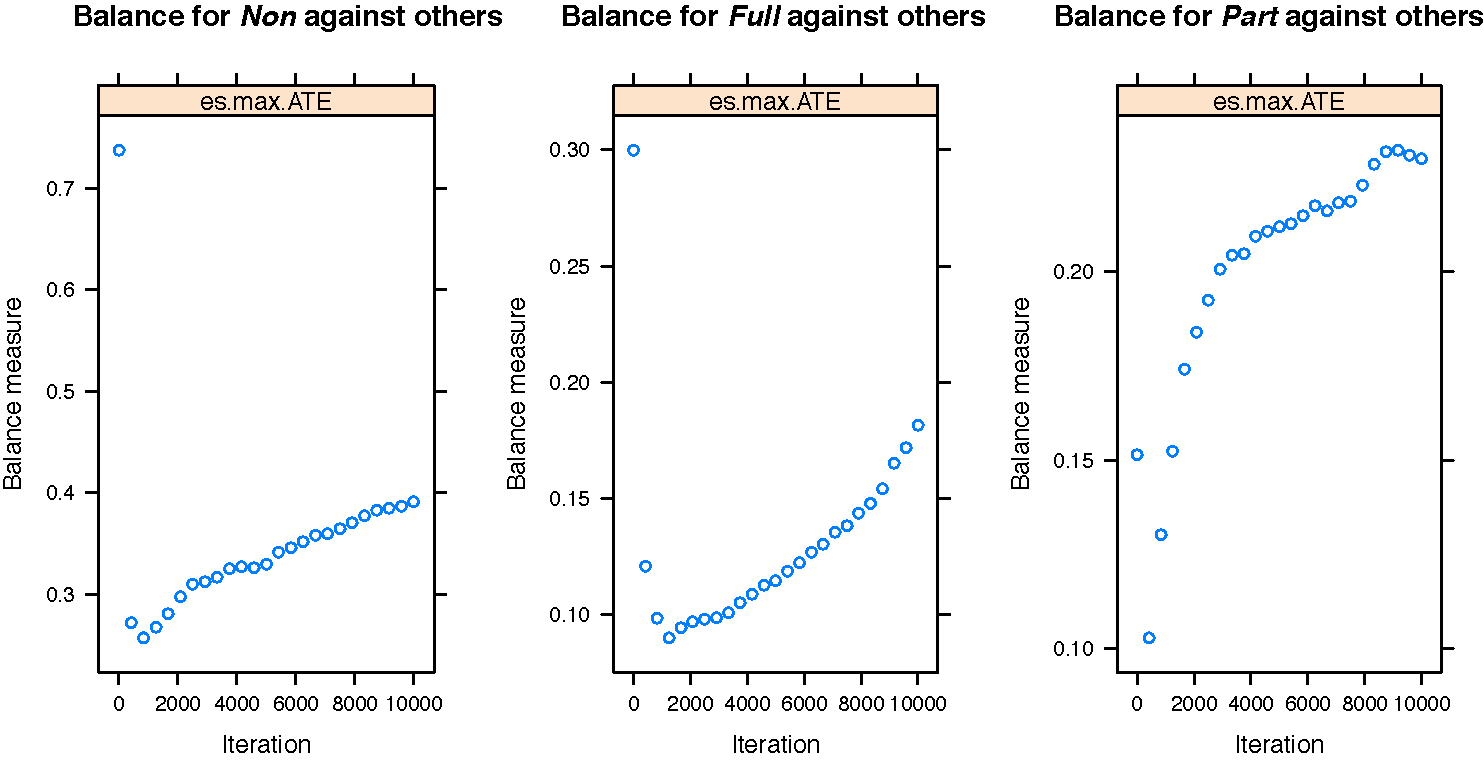
\includegraphics[width=\textwidth]{psdiag1.pdf}
\caption{{\bf GBM iterations and balance measure}}
\label{fig:diag1}
\end{center}
\end{figure}

\subsection{Overlapping assumption satisfied}
One key assumption of propensity score analysis is the overlapping assumption. Propensity score analyses assume that each experiment unit has a non-zero probability of receiving each treatment \citep{mnps2015}. We can examine the plausibility of this assumption by evaluating the overlap of the empirical propensity score distribution. As shown in the Figure \ref{fig:diag2}, although physicians who fully adopted EHR have a higher possibility of being in this treatment group, the overlap assumption generally seems to be met for each treatment group. 

\begin{figure}[!htb]
\begin{center}
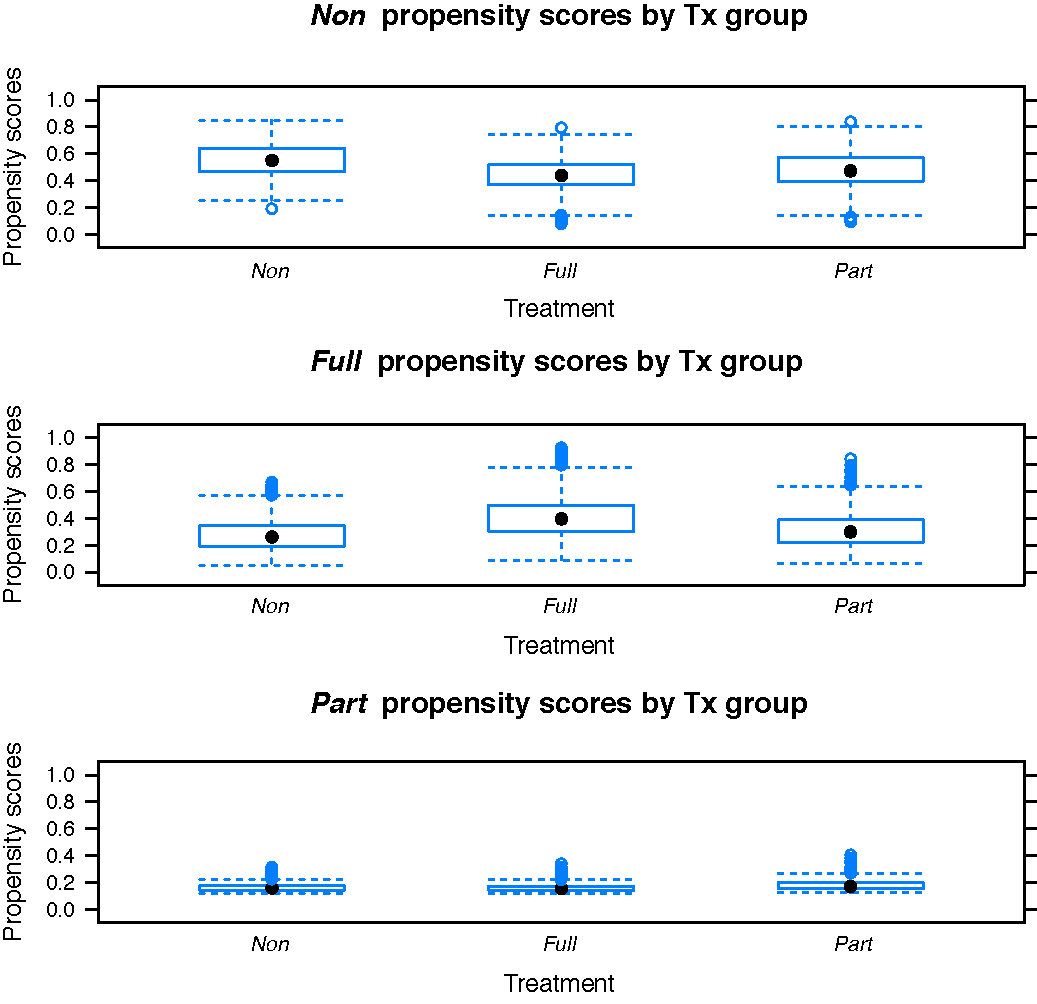
\includegraphics[width=\textwidth]{psdiag2.pdf}
\caption{{\bf Propensity score overlapping assumption}}
\label{fig:diag2}
\end{center}
\end{figure}

\subsection{Propensity score balance achieved}
Figure \ref{fig:diag3} and Figure \ref{fig:diag4} graphically summarize balance statistics from propensity score estimated with a GBM model. In our analysis, each treatment variable of interest has three ASMD statistics, including the difference between non-adopted and fully adopted, the difference between non-adopted and partially adopted, and the difference between partially adopted and fully adopted. Figure \ref{fig:diag3} collapses these three statistics to covariate level and provides an overall comparison of the ASMD between each group before and after weighting. Figure \ref{fig:diag4} assesses the balance before and after weighting for each treatment group.The statistically significant difference is indicated by the solid circle.

As shown in Figure \ref{fig:diag3}, covariates in unbalanced data are highly unbalanced. After weighting, the maximum ASMDs significantly decrease for highly unbalanced variables. Some well-balanced variables have slightly worse balances after weighting because those variables do not predict treatment, leading to relatively random matching on them. As shown in the figure, the ASMDs$<0.25$ criterion is easily met for all pretreatment variables after propensity score weighting. Some variates have an ASMD greater than 0.1, which will be included in regression analysis later to achieve ``double robustness.''


\begin{figure}[!htb]
\begin{center}
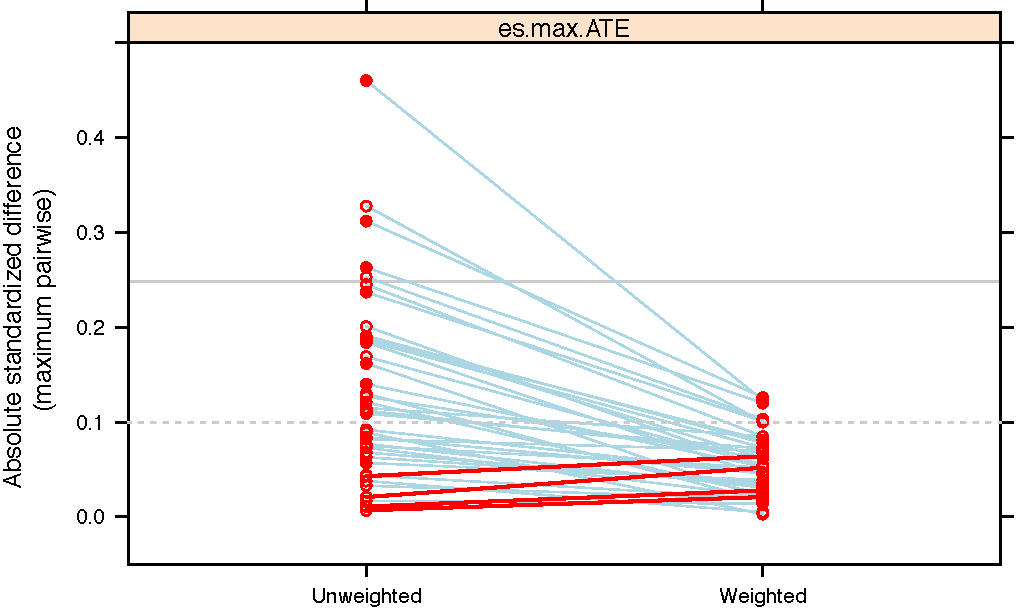
\includegraphics[width=\textwidth]{psdiag3.pdf}
\caption{{\bf Propensity score balancing}}
\label{fig:diag3}
\end{center}
\end{figure}

As shown in Figure \ref{fig:diag4}, observed covariates are well balanced between each possible pair of treatments in our analysis. Figure \ref{fig:diag4} illustrates the difference in maximum ASMDs by treatment group before and after propensity score weighting. Physician practices in different treatment groups have heterogeneous characteristics before the propensity score weighting procedure, especially between those who have fully adopted the EHR and those who have no EHR adoption (see left panel). Only one variable has not reached an ASMD below 0.1 with statistical difference among all pairwise comparisons (see solid dot in weighted data, left panel). Although a few variables exceed the 0.1 ASMD threshold in the middle and right panel, non of them are statistically significant. All variables in three treatment groups have less than 0.25 ASMD after propensity score weighting.

\begin{figure}[!htb]
\begin{center}
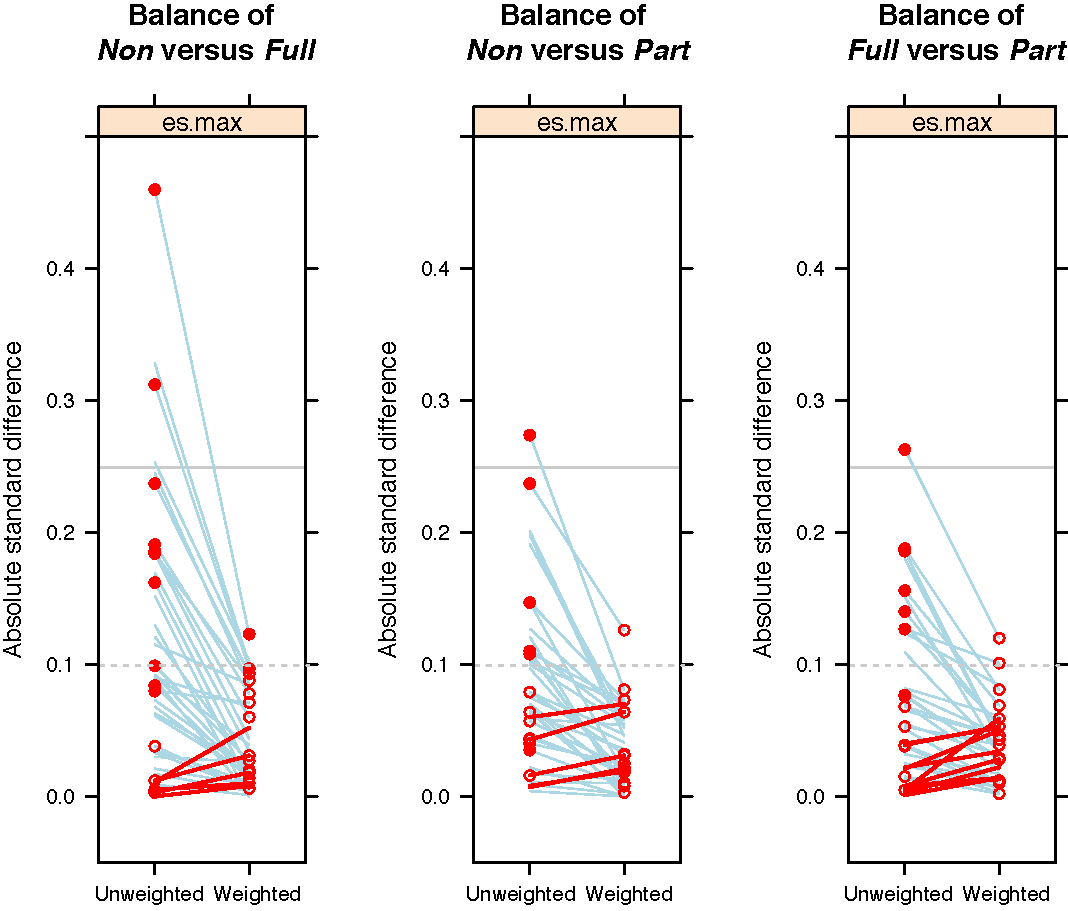
\includegraphics[width=\textwidth]{psdiag4.pdf}
\caption{{\bf Propensity score balancing by treatment group}}
\label{fig:diag4}
\end{center}
\end{figure}

\section{Tabular assessments of balance}
Table \ref{tab:ess} shows the effective sample size (ESS) before and after propensity score weighting. The ESS is approximately the number of observations from a simple random sample that yields an estimate with sampling variation equal to the sampling variation obtained with the weighted comparison observations \citep{twangvignettes}.  Overall, the effective sample size has reduced to 60.86\% of the sample without propensity score weighting. While this may seem like a large loss in sample size, this indicates that many of the physicians were observably unlike their counterparts in different treatment groups and, hence, were not useful for isolating the treatment effect of the EHR system.

\begin{table}[h]
\caption{Effective sample size by treatment group}
\centering
\footnotesize
\label{tab:ess}
\begin{tabular}{lccc}
\hline \hline
Treatment & n    & ESS        & Proportion \\ \hline
Non       & 1853 & 1,116.9608 & 0.6028     \\
Full      & 1146 & 695.7736   & 0.6071     \\
Part      & 620  & 389.6171   & 0.6284     \\
          &     &               &           \\
All       & 3619 & 2,202.3515 & 0.6086     \\ \hline \hline 
\end{tabular}
\end{table}

Table \ref{tab:psbalance} shows the maximum ASMDs of each covariate before and after propensity score weighting. Before propensity score weighting, the maximum ASMDs is 0.4605, which exceeds the 0.25 threshold and is considered unacceptable. Only a few characteristics of physician practices are well balanced with maximum ASMDs less than 0.1, including MSA status and average patient age, etc. The ownership type, physician specialities, solo status, and year of visit are highly unbalanced with maximum ASMDs greater than 0.25. 

The propensity score weighting procedure significantly improves the balance between each treatment group. The maximum ASMD in weighted sample is 0.1259, far below the 0.25 threshold. Few variables have maximum ASMDs greater than 0.10 after weighting, including ownership type, managed care contracts, solo status, and visit year. MSA status, physician specialties, region, patient chronological conditions, physician age, and patient insurance type are considered to be well balanced with ASMDs less than 0.1.



Although the observed covariates balanced relatively well, it is possible that unobserved differences between each two of three groups could still remain.


{\footnotesize
\begin{center}
\label{tab:psbalance}

\renewcommand*{\arraystretch}{0.6}
\begin{longtable}{lSS[table-format = 0.4]}
\caption{Propensity score balance statistics}\\

\hline \hline
Variable                               & \multicolumn{1}{p{3cm}}{\centering Max Std. ES \\(UNW)} & \multicolumn{1}{p{3cm}}{\centering Max Std. ES \\(PSW)} \\  \hline \endfirsthead

\caption*{Propensity Score Balance Statistics (Cont'd)}\\

\hline 
Variable                               & \multicolumn{1}{p{3cm}}{\centering Max Std. ES \\(UNW)} & \multicolumn{1}{p{3cm}}{\centering Max Std. ES \\(PSW)} \\  \hline \endhead

\hline  \multicolumn{3}{r}{\textit{table continues}}\\ \endfoot
\hline \hline  \textit{Note:} $^{*}$ Std. ES $>0.1000$, $^{***}$ Std. ES $>$0.2500 \endlastfoot


                                       &                          &                           \\
\textbf{Ownership Type}                &                          &                           \\
Physician or physician group           & 0.3123$^{***}$               & 0.1259$^{*}$                \\
Health Maintenance Organization (HMO)  & 0.2530$^{***}$               & 0.1033$^{*}$                \\
Community health center                & 0.1089$^{*}$               & 0.0725                    \\
Medical/academic health center         & 0.0680                   & 0.0337                    \\
Other hospital                         & 0.0754                   & 0.0524                    \\
Other health care corporation          & 0.1693$^{*}$               & 0.0549                    \\
Other                                  & 0.0922                   & 0.0470                    \\
                                       &                          &                           \\
\textbf{Metropolitan Statistical Area} &                          &                           \\
MSA                                    & 0.0427                   & 0.0643                    \\
Non-MSA                                & 0.0427                   & 0.0643                    \\
                                       &                          &                           \\
\textbf{Managed Care Contracts}        &                          &                           \\
None                                   & 0.2372$^{*}$               & 0.1006$^{*}$                \\
Less than 3                            & 0.0111                   & 0.0285                    \\
3 - 10                                 & 0.1209$^{*}$               & 0.0235                    \\
Greater than 10                        & 0.2452$^{*}$               & 0.0853                    \\
                                       &                          &                           \\
\textbf{Physician specialties}         &                          &                           \\
General/family practice                & 0.1913$^{*}$               & 0.0776                    \\
Internal medicine                      & 0.0818                   & 0.0702                    \\
Pediatrics                             & 0.0167                   & 0.0145                    \\
General surgery                        & 0.0893                   & 0.0032                    \\
Obstetrics and gynecology              & 0.0070                   & 0.0208                    \\
Orthopedic surgery                     & 0.0632                   & 0.0364                    \\
Cardiovascular diseases                & 0.2011$^{*}$               & 0.0520                    \\
Dermatology                            & 0.1907$^{*}$               & 0.0615                    \\
Urology                                & 0.0730                   & 0.0219                    \\
Psychiatry                             & 0.3280$^{***}$               & 0.0998                    \\
Neurology                              & 0.1297$^{*}$               & 0.0168                    \\
Ophthalmology                          & 0.1840$^{*}$               & 0.0435                    \\
Otolaryngology                         & 0.0384                   & 0.0048                    \\
Other specialties                      & 0.0206                   & 0.0516                    \\
Oncology                               & 0.1266$^{*}$               & 0.0624                    \\
                                       &                          &                           \\
\textbf{Solo}                                   & 0.4605$^{***}$               & 0.1233$^{*}$                \\
                                       &                          &                           \\
\textbf{Region}                        &                          &                           \\
Northeast                              & 0.0568                   & 0.0395                    \\
Midwest                                & 0.1122$^{*}$               & 0.0680                    \\
South                                  & 0.0331                   & 0.0191                    \\
West                                   & 0.1146$^{*}$               & 0.0850                    \\
                                       &                          &                           \\
\textbf{Avg. chron cond.}              & 0.1618$^{*}$               & 0.0199                    \\
\textbf{Avg. patient age}              & 0.0768                   & 0.0306                    \\
                                       &                          &                           \\
\textbf{Patient insurance type}        &                          &                           \\
Private insurance                      & 0.0837                   & 0.0457                    \\
Medicare                               & 0.1882$^{*}$               & 0.0815                    \\
Medicaid                               & 0.1398$^{*}$               & 0.0526                    \\
Workers Compensation                   & 0.0440                   & 0.0199                    \\
Self-pay                               & 0.1860$^{*}$               & 0.0727                    \\
                                       &                          &                           \\
\textbf{Visit Year}                    & 0.2630$^{***}$               & 0.1199$^{*}$    \\

\end{longtable}
\end{center}}

\chapter{Regression results}
\label{chapter: reg}

\section{Model specification}
In our analysis, we use eight models to assess the effect of EHR adoption on patient-specific health education prescription rate, time utilization, and returned appointment rate. As discussed in Chapter \ref{sec:model} and Chapter \ref{sec:spec}, we mainly focus on results in Model (1) in Table \ref{tab:edu}, Table \ref{tab:time}, and Table \ref{tab:return}. Model (1) is a generalized linear regression model weighted by a multinomial propensity score and only controlled covariates with ASMD$>$0.1, of each outcome. 

Models (2) through (8) in Table \ref{tab:edu}, Table \ref{tab:time}, and Table \ref{tab:return} serve as sensitivity tests of Model (1). Model (2) has the same model specification with Model (1), but use binomial or poisson regression depending on the dependent variable's distribution. Model (3) and Model (4) have the same multinomial propensity score with Model (1) while Model (3) includes no covariates and Model (4) includes all covariates. Model (5) through Model (8) use binary treatment assignment instead of multiple treatment assignments in propensity score estimation and regression adjustment. Model (5) and Model (6) estimate the treatment effect of full EHR adoption and partial EHR adoption with propensity score weighting. Model (7) and Model (8) analyze that with propensity score matching. 

\section{EHR adoption has a positive effect on patient-specific health education prescription rates}
Table \ref{tab:edu} illustrates the effect of EHR adoption on patient-specific health education prescription rates. 

As shown in Model (1), physician practices that have fully adopted the EHR system have statistically significant higher patient-specific health education prescription rates than their counterparts at a 90\% confidence level. Physicians are expected to increase patient-specific health education prescription rates by 3.4\% if they fully adopt the EHR system. This result is robust among different regression models, with no substantial difference. However, there are no statistically significant relationships between partial EHR adoption and patient-specific health education prescription rates. 

Physicians can identify patient-specific education resources through integrated programs with certified EHR technology. The EHR system can use the patient's demographic characteristics, diagnostics and medications, or other patient information to suggest education resources that would be of value to the patient \citep{hitrc_edu}. 

\section{EHR adoption has no effect on time utilization}
Table \ref{tab:time} demonstrates the estimated effect of EHR adoption on physician-patient interaction time. As shown in Model (1), there are no statistically significant relationships between full or partial EHR adoption and time utilization. The sign of coefficients is mixed among different model specifications.

Similar to physician practices that have fully adopted the EHR system, physician practices that have partially adopted the EHR system also have no statistically significant effects on time utilization. Coefficients have mixed signs among different model specifications.



\section{EHR adoption has no robust effect on returned appointment rates}

Table \ref{tab:return} shows the estimated effect of EHR adoption on the returned appointment rate. Physician practices that have fully adopted the EHR system have fewer returned appointments. The returned appointment is expected to decrease by 0.31\% if the physician practices have the full EHR adoption. 

There are no statistically significant relationships between physician practices that have partially adopted the EHR system and returned appointment rate. The sign of coefficients shows that partial EHR adoption in physician practices \textit{may} reduce the returned appointment rate, but the coefficient is not statistically significant.

Although Model (1) suggests that there are statistically significant relationships between full EHR adoption and the returned appointment rate; it is not robust with different model specifications.  As shown in Model (4) and Model (7), there are no statistically significant relationships between EHR adoption and returned appointment rate with different model specifications.

\begin{landscape}
\begin{table}[p] \centering 
  \caption{Estimated effect of EHR adoption on patient-specific health education prescription rates} 
  \label{tab:edu} 
\footnotesize 
\begin{tabular}{@{\extracolsep{-15pt}}lD{.}{.}{-3} D{.}{.}{-3} D{.}{.}{-3} D{.}{.}{-3} D{.}{.}{-3} D{.}{.}{-3} D{.}{.}{-3} D{.}{.}{-3} } 
\\[-1.8ex]\hline 
\hline \\[-1.8ex] 
 & \multicolumn{8}{c}{\textit{Dependent variable: patient-specific health education prescription rates}} \\ 
\cline{2-9} 
\\[-1.8ex] & \multicolumn{1}{c}{(1)} & \multicolumn{1}{c}{(2)} & \multicolumn{1}{c}{(3)} & \multicolumn{1}{c}{(4)} & \multicolumn{1}{c}{(5)} & \multicolumn{1}{c}{(6)} & \multicolumn{1}{c}{(7)} & \multicolumn{1}{c}{(8)}\\ 
\hline \\[-1.8ex] 
Full EHR & 0.034^{*} & 0.143^{*} & 0.037^{**} & 0.034^{**} & 0.043^{**} &  & 0.039^{***} &  \\ 
  & (0.018) & (0.074) & (0.018) & (0.017) & (0.019) &  & (0.015) &  \\ 
Part EHR & 0.033 & 0.135 & 0.034^{*} & 0.034^{*} &  & 0.028 &  & 0.006 \\ 
  & (0.020) & (0.084) & (0.020) & (0.019) &  & (0.021) &  & (0.020) \\ 
  Constant & 0.411^{***} & -0.363^{***} & 0.401^{***} & 0.334^{***} & 0.405^{***} & 0.363^{***} & 0.401^{***} & 0.344^{***} \\ 
  & (0.031) & (0.128) & (0.010) & (0.064) & (0.035) & (0.034) & (0.027) & (0.035) \\ 
 \\ [-1.8ex]\hline

Treatment & \multicolumn{1}{c}{\textit{Multiple}}& \multicolumn{1}{c}{\textit{Multiple}}& \multicolumn{1}{c}{\textit{Multiple}}& \multicolumn{1}{c}{\textit{Multiple}}& \multicolumn{1}{c}{\textit{Binary}}&\multicolumn{1}{c}{\textit{Binary}}&\multicolumn{1}{c}{\textit{Binary}}&\multicolumn{1}{c}{\textit{Binary}}\\
PS & \multicolumn{1}{c}{\textit{Weighting}}& \multicolumn{1}{c}{\textit{Weighting}}& \multicolumn{1}{c}{\textit{Weighting}}& \multicolumn{1}{c}{\textit{Weighting}}& \multicolumn{1}{c}{\textit{Weighting}}&\multicolumn{1}{c}{\textit{Weighting}}&\multicolumn{1}{c}{\textit{Matching}}&\multicolumn{1}{c}{\textit{Matching}}\\
Controlled ASMD $>$0.1 & \multicolumn{1}{c}{\textit{Yes}}& \multicolumn{1}{c}{\textit{Yes}}& \multicolumn{1}{c}{\textit{No}}& \multicolumn{1}{c}{\textit{Yes}}& \multicolumn{1}{c}{\textit{Yes}}&\multicolumn{1}{c}{\textit{Yes}}&\multicolumn{1}{c}{\textit{Yes}}&\multicolumn{1}{c}{\textit{Yes}}\\
Controlled ASMD $<$0.1 & \multicolumn{1}{c}{\textit{No}}& \multicolumn{1}{c}{\textit{No}}& \multicolumn{1}{c}{\textit{No}}& \multicolumn{1}{c}{\textit{Yes}}& \multicolumn{1}{c}{\textit{No}}&\multicolumn{1}{c}{\textit{No}}&\multicolumn{1}{c}{\textit{No}}&\multicolumn{1}{c}{\textit{No}}\\
Error dist. & \multicolumn{1}{c}{\textit{Normal}}& \multicolumn{1}{c}{\textit{Binomial}}& \multicolumn{1}{c}{\textit{Normal}}& \multicolumn{1}{c}{\textit{Normal}}& \multicolumn{1}{c}{\textit{Normal}}&\multicolumn{1}{c}{\textit{Normal}}&\multicolumn{1}{c}{\textit{Normal}}&\multicolumn{1}{c}{\textit{Normal}}\\
\\ [-1.8ex]\hline
Observations & \multicolumn{1}{c}{3,619} & \multicolumn{1}{c}{3,619} & \multicolumn{1}{c}{3,619} & \multicolumn{1}{c}{3,619} & \multicolumn{1}{c}{2,999} & \multicolumn{1}{c}{2,473} & \multicolumn{1}{c}{2,292} & \multicolumn{1}{c}{1,240} \\ 
R$^{2}$ &  &  &  &  &  &  & \multicolumn{1}{c}{0.017} & \multicolumn{1}{c}{0.028} \\ 
Adjusted R$^{2}$ &  &  &  &  &  &  & \multicolumn{1}{c}{0.011} & \multicolumn{1}{c}{0.017} \\ 
Log Likelihood & \multicolumn{1}{c}{-2,048.801} &  & \multicolumn{1}{c}{-2,072.498} & \multicolumn{1}{c}{-1,853.567} & \multicolumn{1}{c}{-1,613.901} & \multicolumn{1}{c}{-1,385.733} &  &  \\ 
Akaike Inf. Crit. & \multicolumn{1}{c}{4,127.603} &  & \multicolumn{1}{c}{4,150.996} & \multicolumn{1}{c}{3,787.134} & \multicolumn{1}{c}{3,255.802} & \multicolumn{1}{c}{2,799.466} &  &  \\ 
Residual Std. Error &  &  &  &  &  &  & \multicolumn{1}{c}{0.340} & \multicolumn{1}{c}{0.347} \\ 
 &  &  &  &  &  &  & \multicolumn{1}{c}{(df = 2278)} & \multicolumn{1}{c}{(df = 1226)} \\ 
F Statistic &  &  &  &  &  &  & \multicolumn{1}{c}{2.942$^{***}$ } & \multicolumn{1}{c}{2.675$^{***}$} \\ 
&  &  &  &  &  &  & \multicolumn{1}{c}{(df = 13; 2278)} & \multicolumn{1}{c}{(df = 13; 1226)} \\ 
\hline 
\hline \\[-1.8ex] 
 \multicolumn{9}{l}{\textit{Note:Standard errors are reported in parentheses.} $^{*}$p$<$0.1; $^{**}$p$<$0.05; $^{***}$p$<$0.01} \\ 
\end{tabular} 
\end{table} 
\end{landscape}

% Table created by stargazer v.5.1 by Marek Hlavac, Harvard University. E-mail: hlavac at fas.harvard.edu
% Date and time: Sun, Mar 29, 2015 - 11:35:58
% Requires LaTeX packages: dcolumn
\begin{landscape} 
\begin{table}[p] \centering 
  \caption{Estimated effect of EHR adoption on patient-physician interaction time} 
  \label{tab:time} 
\footnotesize 
\begin{tabular}{@{\extracolsep{-15pt}}lD{.}{.}{-3} D{.}{.}{-3} D{.}{.}{-3} D{.}{.}{-3} D{.}{.}{-3} D{.}{.}{-3} D{.}{.}{-3} D{.}{.}{-3} } 
\\[-1.8ex]\hline 
\hline \\[-1.8ex] 
 & \multicolumn{8}{c}{\textit{Dependent variable: patient-physician interaction time}} \\ 
\cline{2-9} 
\\[-1.8ex] & \multicolumn{1}{c}{(1)} & \multicolumn{1}{c}{(2)} & \multicolumn{1}{c}{(3)} & \multicolumn{1}{c}{(4)} & \multicolumn{1}{c}{(5)} & \multicolumn{1}{c}{(6)} & \multicolumn{1}{c}{(7)} & \multicolumn{1}{c}{(8)}\\ 
\hline \\[-1.8ex] 
Full EHR & 0.222 & 0.010 & -0.038 & 0.353 & 0.319 &  & 0.475 &  \\ 
  & (0.532) & (0.024) & (0.538) & (0.472) & (0.568) &  & (0.403) &  \\ 
Part EHR & 0.189 & 0.007 & 0.054 & 0.213 &  & 0.122 &  & -0.125 \\ 
  & (0.574) & (0.026) & (0.593) & (0.519) &  & (0.605) &  & (0.554) \\ 
  Constant & 25.074^{***} & 3.213^{***} & 21.821^{***} & 20.295^{***} & 25.938^{***} & 25.420^{***} & 23.439^{***} & 24.723^{***} \\ 
  & (1.102) & (0.044) & (0.345) & (2.247) & (1.297) & (1.383) & (0.743) & (0.964) \\ 
 \hline \\[-1.8ex] 
 Treatment & \multicolumn{1}{c}{\textit{Multiple}}& \multicolumn{1}{c}{\textit{Multiple}}& \multicolumn{1}{c}{\textit{Multiple}}& \multicolumn{1}{c}{\textit{Multiple}}& \multicolumn{1}{c}{\textit{Binary}}&\multicolumn{1}{c}{\textit{Binary}}&\multicolumn{1}{c}{\textit{Binary}}&\multicolumn{1}{c}{\textit{Binary}}\\
PS & \multicolumn{1}{c}{\textit{Weighting}}& \multicolumn{1}{c}{\textit{Weighting}}& \multicolumn{1}{c}{\textit{Weighting}}& \multicolumn{1}{c}{\textit{Weighting}}& \multicolumn{1}{c}{\textit{Weighting}}&\multicolumn{1}{c}{\textit{Weighting}}&\multicolumn{1}{c}{\textit{Matching}}&\multicolumn{1}{c}{\textit{Matching}}\\
Controlled ASMD $>$0.1 & \multicolumn{1}{c}{\textit{Yes}}& \multicolumn{1}{c}{\textit{Yes}}& \multicolumn{1}{c}{\textit{No}}& \multicolumn{1}{c}{\textit{Yes}}& \multicolumn{1}{c}{\textit{Yes}}&\multicolumn{1}{c}{\textit{Yes}}&\multicolumn{1}{c}{\textit{Yes}}&\multicolumn{1}{c}{\textit{Yes}}\\
Controlled ASMD $<$0.1 & \multicolumn{1}{c}{\textit{No}}& \multicolumn{1}{c}{\textit{No}}& \multicolumn{1}{c}{\textit{No}}& \multicolumn{1}{c}{\textit{Yes}}& \multicolumn{1}{c}{\textit{No}}&\multicolumn{1}{c}{\textit{No}}&\multicolumn{1}{c}{\textit{No}}&\multicolumn{1}{c}{\textit{No}}\\
Error dist. & \multicolumn{1}{c}{\textit{Normal}}& \multicolumn{1}{c}{\textit{Poisson}}& \multicolumn{1}{c}{\textit{Normal}}& \multicolumn{1}{c}{\textit{Normal}}& \multicolumn{1}{c}{\textit{Normal}}&\multicolumn{1}{c}{\textit{Normal}}&\multicolumn{1}{c}{\textit{Normal}}&\multicolumn{1}{c}{\textit{Normal}}\\
\\ [-1.8ex]\hline

Observations & \multicolumn{1}{c}{3,619} & \multicolumn{1}{c}{3,619} & \multicolumn{1}{c}{3,619} & \multicolumn{1}{c}{3,619} & \multicolumn{1}{c}{2,999} & \multicolumn{1}{c}{2,473} & \multicolumn{1}{c}{2,292} & \multicolumn{1}{c}{1,240} \\ 
R$^{2}$ &  &  &  &  &  &  & \multicolumn{1}{c}{0.053} & \multicolumn{1}{c}{0.078} \\ 
Adjusted R$^{2}$ &  &  &  &  &  &  & \multicolumn{1}{c}{0.048} & \multicolumn{1}{c}{0.068} \\ 
Log Likelihood & \multicolumn{1}{c}{-14,216.760} &  & \multicolumn{1}{c}{-14,331.300} & \multicolumn{1}{c}{-13,858.460} & \multicolumn{1}{c}{-11,843.320} & \multicolumn{1}{c}{-9,902.171} &  &  \\ 
Akaike Inf. Crit. & \multicolumn{1}{c}{28,463.530} &  & \multicolumn{1}{c}{28,668.600} & \multicolumn{1}{c}{27,796.920} & \multicolumn{1}{c}{23,714.630} & \multicolumn{1}{c}{19,832.340} &  &  \\ 
Residual Std. Error &  &  &  &  &  &  & \multicolumn{1}{c}{9.203} & \multicolumn{1}{c}{9.468} \\ 
 &  &  &  &  &  &  & \multicolumn{1}{c}{(df = 2278)} & \multicolumn{1}{c}{(df = 1226)} \\ 
F Statistic &  &  &  &  &  &  & \multicolumn{1}{c}{9.895$^{***}$} & \multicolumn{1}{c}{8.006$^{***}$} \\ 
 &  &  &  &  &  &  & \multicolumn{1}{c}{(df = 13; 2278)} & \multicolumn{1}{c}{(df = 13; 1226)} \\ 
\hline 
\hline \\[-1.8ex] 
 \multicolumn{9}{l}{\textit{Note:Standard errors are reported in parentheses.} $^{*}$p$<$0.1; $^{**}$p$<$0.05; $^{***}$p$<$0.01} \\ 

\end{tabular} 
\end{table}
\end{landscape}

% Table created by stargazer v.5.1 by Marek Hlavac, Harvard University. E-mail: hlavac at fas.harvard.edu
% Date and time: Sun, Mar 29, 2015 - 11:42:05
% Requires LaTeX packages: dcolumn 
\begin{landscape} 
\begin{table}[p] \centering 
  \caption{Estimated effect of EHR adoption on returned appointment rates} 
  \label{tab:return} 
\footnotesize 
\begin{tabular}{@{\extracolsep{-15pt}}lD{.}{.}{-3} D{.}{.}{-3} D{.}{.}{-3} D{.}{.}{-3} D{.}{.}{-3} D{.}{.}{-3} D{.}{.}{-3} D{.}{.}{-3} } 
\\[-1.8ex]\hline 
\hline \\[-1.8ex] 
 & \multicolumn{8}{c}{\textit{Dependent variable: returned appointment rates}} \\ 
\cline{2-9} 
\\[-1.8ex] & \multicolumn{1}{c}{(1)} & \multicolumn{1}{c}{(2)} & \multicolumn{1}{c}{(3)} & \multicolumn{1}{c}{(4)} & \multicolumn{1}{c}{(5)} & \multicolumn{1}{c}{(6)} & \multicolumn{1}{c}{(7)} & \multicolumn{1}{c}{(8)}\\ 
\hline \\[-1.8ex] 
Full EHR & -0.031^{**} & -0.150^{**} & -0.035^{**} & -0.020 & -0.030^{**} &  & -0.011 &  \\ 
  & (0.015) & (0.070) & (0.014) & (0.013) & (0.015) &  & (0.012) &  \\ 
Part EHR & -0.008 & -0.038 & -0.011 & -0.012 &  & -0.002 &  & 0.020 \\ 
  & (0.018) & (0.086) & (0.018) & (0.016) &  & (0.017) &  & (0.016) \\ 
  Constant & 0.679^{***} & 0.747^{***} & 0.719^{***} & 0.392^{***} & 0.696^{***} & 0.694^{***} & 0.678^{***} & 0.683^{***} \\ 
  & (0.026) & (0.125) & (0.009) & (0.055) & (0.027) & (0.028) & (0.023) & (0.028) \\ 
 \hline \\[-1.8ex] 
  Treatment & \multicolumn{1}{c}{\textit{Multiple}}& \multicolumn{1}{c}{\textit{Multiple}}& \multicolumn{1}{c}{\textit{Multiple}}& \multicolumn{1}{c}{\textit{Multiple}}& \multicolumn{1}{c}{\textit{Binary}}&\multicolumn{1}{c}{\textit{Binary}}&\multicolumn{1}{c}{\textit{Binary}}&\multicolumn{1}{c}{\textit{Binary}}\\
PS & \multicolumn{1}{c}{\textit{Weighting}}& \multicolumn{1}{c}{\textit{Weighting}}& \multicolumn{1}{c}{\textit{Weighting}}& \multicolumn{1}{c}{\textit{Weighting}}& \multicolumn{1}{c}{\textit{Weighting}}&\multicolumn{1}{c}{\textit{Weighting}}&\multicolumn{1}{c}{\textit{Matching}}&\multicolumn{1}{c}{\textit{Matching}}\\
Controlled ASMD $>$0.1 & \multicolumn{1}{c}{\textit{Yes}}& \multicolumn{1}{c}{\textit{Yes}}& \multicolumn{1}{c}{\textit{No}}& \multicolumn{1}{c}{\textit{Yes}}& \multicolumn{1}{c}{\textit{Yes}}&\multicolumn{1}{c}{\textit{Yes}}&\multicolumn{1}{c}{\textit{Yes}}&\multicolumn{1}{c}{\textit{Yes}}\\
Controlled ASMD $<$0.1 & \multicolumn{1}{c}{\textit{No}}& \multicolumn{1}{c}{\textit{No}}& \multicolumn{1}{c}{\textit{No}}& \multicolumn{1}{c}{\textit{Yes}}& \multicolumn{1}{c}{\textit{No}}&\multicolumn{1}{c}{\textit{No}}&\multicolumn{1}{c}{\textit{No}}&\multicolumn{1}{c}{\textit{No}}\\
Error dist. & \multicolumn{1}{c}{\textit{Normal}}& \multicolumn{1}{c}{\textit{Binomial}}& \multicolumn{1}{c}{\textit{Normal}}& \multicolumn{1}{c}{\textit{Normal}}& \multicolumn{1}{c}{\textit{Normal}}&\multicolumn{1}{c}{\textit{Normal}}&\multicolumn{1}{c}{\textit{Normal}}&\multicolumn{1}{c}{\textit{Normal}}\\
\\ [-1.8ex]\hline

Observations & \multicolumn{1}{c}{3,619} & \multicolumn{1}{c}{3,619} & \multicolumn{1}{c}{3,619} & \multicolumn{1}{c}{3,619} & \multicolumn{1}{c}{2,999} & \multicolumn{1}{c}{2,473} & \multicolumn{1}{c}{2,292} & \multicolumn{1}{c}{1,240} \\ 
R$^{2}$ &  &  &  &  &  &  & \multicolumn{1}{c}{0.018} & \multicolumn{1}{c}{0.017} \\ 
Adjusted R$^{2}$ &  &  &  &  &  &  & \multicolumn{1}{c}{0.013} & \multicolumn{1}{c}{0.007} \\ 
Log Likelihood & \multicolumn{1}{c}{-1,394.416} &  & \multicolumn{1}{c}{-1,423.651} & \multicolumn{1}{c}{-1,011.757} & \multicolumn{1}{c}{-1,101.507} & \multicolumn{1}{c}{-911.617} &  &  \\ 
Akaike Inf. Crit. & \multicolumn{1}{c}{2,818.832} &  & \multicolumn{1}{c}{2,853.302} & \multicolumn{1}{c}{2,103.514} & \multicolumn{1}{c}{2,231.015} & \multicolumn{1}{c}{1,851.235} &  &  \\ 
Residual Std. Error &  &  &  &  &  &  & \multicolumn{1}{c}{0.284 } & \multicolumn{1}{c}{0.277} \\ 
 &  &  &  &  &  &  & \multicolumn{1}{c}{(df = 2278)} & \multicolumn{1}{c}{(df = 1226)} \\ 
F Statistic &  &  &  &  &  &  & \multicolumn{1}{c}{3.251$^{***}$} & \multicolumn{1}{c}{1.649$^{*}$} \\ 
F Statistic &  &  &  &  &  &  & \multicolumn{1}{c}{(df = 13; 2278)} & \multicolumn{1}{c}{(df = 13; 1226)} \\ 
\hline 
\hline \\[-1.8ex] 
 \multicolumn{9}{l}{\textit{Note:Standard errors are reported in parentheses.} $^{*}$p$<$0.1; $^{**}$p$<$0.05; $^{***}$p$<$0.01} \\ 

\end{tabular} 
\end{table} 
\end{landscape}

\chapter{Discussion}

\label{chapter:discussion}
The federal government has authorized more than \$1.5 billion to provide a financial incentive for EHR adoption. The rationale for this level of expenditure comes from an expectation that the EHR will improve health care quality and efficiency in the United States. In this analysis, we estimate the effect of EHR adoption on the patient-specific education resources prescription rate, time utilization, and returned appointment rates. We find the effect of full EHR adoption on patient-specific health education prescription rates is statistically significant. Physician practices that have full EHR adoption are more likely to prescribe patient-specific health education resources. We do not find statistically significant and robust effects of EHR adoption on time utilization or returned appointment rates.

There are multiple plausible reasons that can explain the EHR's positive effect on patient-specific health education prescription rates. First, patient-specific education resources are easy to prescribe with the EHR system. The certified EHR system automates the process for identifying appropriate education resources. Physicians no longer need to search manually during the consultation. Second, the EHR incentive program has set patient-specific education as a menu objective. To meet this objective, health care providers must provide at least 10\% of patient-specific education resources for patients. There is no exemption for this menu objective. Third, physicians may intentionally use the EHR for shared decision-making and education to improve patient engagement. Physicians can easily share information with patients via the patient portal or printouts, encouraging patients to play an important role in optimizing their treatment outcomes.

Several factors could contribute to a mixed-time utilization outcome after EHR adoption. On the one hand, time efficiency could have improved as physicians became familiar with EHR systems. For example, physicians could check a patient's lab test results or medical histories instantly with the EHR system. On the other hand, certain EHR systems have poor usability. Overwhelming false alert messages and time-consuming data entry could further increase documentation time. Additionally, physicians could have continued to perform certain tasks using paper-based methods, even though the computer automatically performed these tasks for them \citep{overhage2001controlled}.

EHR adoption has a negative (although not robust) effect on returned appointment rates. There are a few hypothetical explanations. First, the EHR system may improve the quality of treatment, and thus, there would be no need to revisit the physician. Second, the patient may disregard the automatic reminder generated by the EHR system. Third is alert fatigue experienced by physicians; they routinely ignore alerts due to the high volume generated by the EHR system. However, testing the plausibility of these hypothetical explanations with our data is difficult.

\chapter{Limitations}
\label{chapter:limitations}
There are limitations to our study that must be considered when interpreting our results.

First, NAMCS data provide information about individual health care encounters. A specific patient who has multiple encounters at the survey site in a certain year has a heavier weight than a counterfactual patient who used health care less frequently. Individuals without any contact with health care providers are not included in the survey. Similarly, physicians who had not interacted with patients are not included in this survey. These may lead to possible selection bias in this analysis.

Second, our casual inference method is based on strong assumptions due to the limitation of observational data. Although NAMCS data provided extensive information about patient demographic and medical information, as well as physician practice information, it is still difficult to satisfy both the stable unit treatment value assumption (SUTVA) and unconfoundedness assumption perfectly. Violations of these assumptions may lead to overestimated or underestimated results.

Third, empirical research on the casual relationship between studied outcomes and health quality is still limited. For example, further analysis is required to detail the effect of received patient-specific education resources on patient compliance.

\chapter{Policy implications}
\label{chapter:policyimplications}
Patients, physicians, administrative agencies, and EHR suppliers all have an interest in improving the usability of EHRs and integrating them into clinical workflows that improve the efficiency and quality of health care. This analysis leads to the following policy implications.

The first is linking patient education with quality improvement efforts. In an effort to improve quality, one goal for health policy should be to ensure a health-literate environment. In such an environment, patients seek health care earlier because they recognize their symptoms, they ask for preventive care to reduce health risks, they understand and follow their doctors' recommendations, and they are not afraid to ask questions if they do not understand. Educating patients with EHR-generated health education materials and physicians' personalized advice are both essential in this process.

Second, the CMS should work with physicians and vendors to improve the usability of EHR systems. Many physicians believe that practice workflow efficiency can be improved by more user-friendly system design. Physicians are looking for an easy-to-use EHR system, such that they can record their encounters better, easier, and faster than they could on paper. Together with physicians and EHR vendors, health policy practitioners should facilitate appropriate certification criteria of EHR systems, which make physicians clinical practices more efficient, more effective, and easier. 

\chapter{Conclusion}
\label{chapter:conclusion}
In summary, we used National Ambulatory Medical Care Survey data to assess whether the ambulatory EHR system is associated with changes in the patient-specific health education prescription rate, patient-physician interaction time, and returned appointment rate. We estimated the treatment effect of full EHR adoption and partial EHR adoption with multinomial propensity score weighting. We found evidence to suggest that full EHR adoption positively affects the patient-specific health education prescription rate. There is no robust evidence to show the effect of the EHR system on time utilization or the returned appointment rate. Linking patient education with quality improvement efforts and improving the usability of EHR systems are both essential to improving health care quality.

\newpage
\bibliographystyle{plainnat}
\bibliography{EHR}

\end{document}
